
\section{Experimental Results and Discussion}

All results were generated with MATLAB running on an i7-2600K 3.4GHz processor.
We used the open source C implementations of kd-trees in VLFeat \cite{picm10VedaldiVLFEAT} and feature extraction from Perdoch{} \cite{cvpr09PerdochEfficRep}.
We were provided with five datasets to test the HotSpotter algorithms.
We thank the Rubenstein team in Kenya for the large Grevy's and plains datasets as well as giraffes; Marcella Kelly for jaguars, and Juan David Gonz\'{a}lez Corredor for lionfish.
Summaries of each are provided in Table~\ref{tab:dbstats}, and examples of each are in Figure~\ref{fig:correctall}.

\subsection{Data Sets}

\newlength{\correctmatchheight}
\setlength{\correctmatchheight}{1.65in}

\begin{figure*}
\begin{center}
\begin{tabular}{c c c c c}
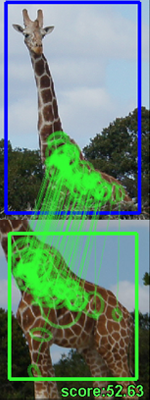
\includegraphics[height=\correctmatchheight]{figures/FinalImages/cropped/GIR_correct_27_cropped2}
&
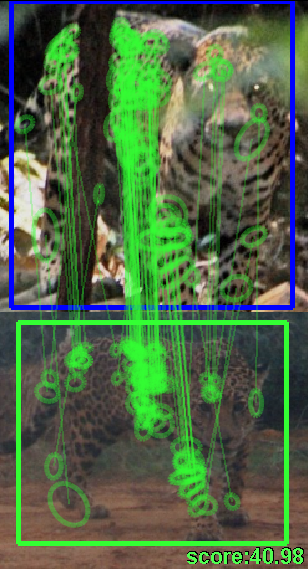
\includegraphics[height=\correctmatchheight]{figures/FinalImages/cropped/JAG_correct_31_cropped}
&
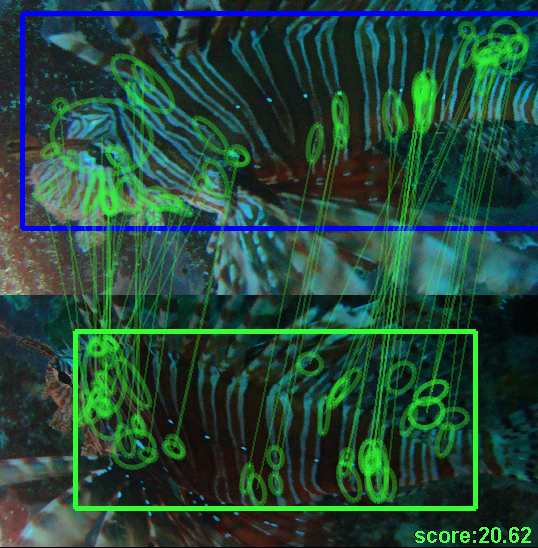
\includegraphics[height=\correctmatchheight]{figures/FinalImages/cropped/LF_correct_14_cropped}
&
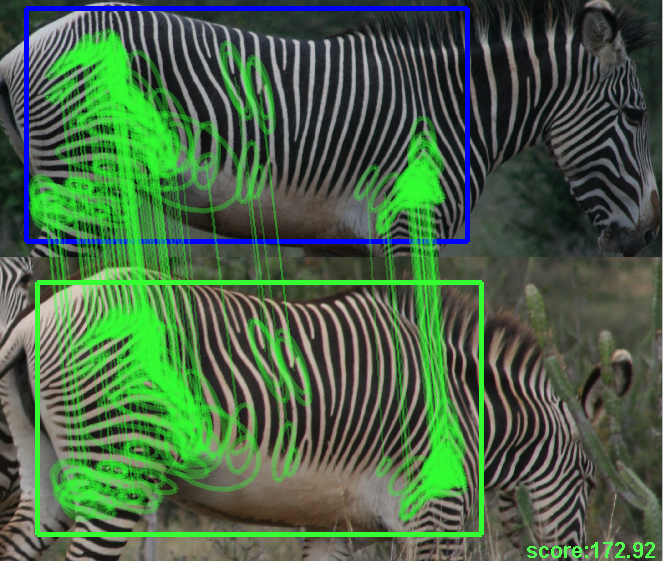
\includegraphics[height=\correctmatchheight]{figures/FinalImages/cropped/GZ_correct_877_cropped}
&
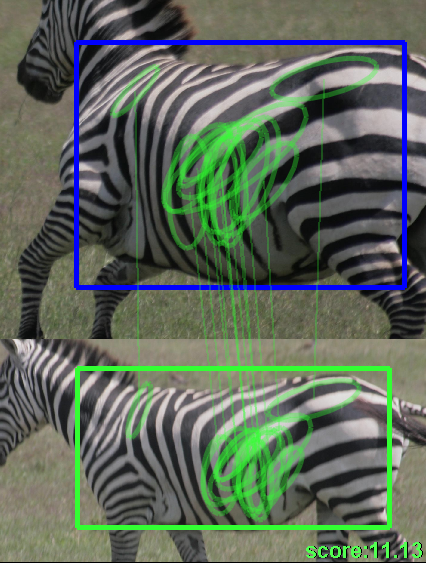
\includegraphics[height=\correctmatchheight]{figures/FinalImages/cropped/PZ_correct_318_cropped}
\end{tabular}
\caption{\footnotesize{Correct matches. The top images are queries and the bottom images are top results. Wild-ID failed on jaguar and lionfish examples.}}
\label{fig:correctall}
\end{center}
\end{figure*}


\begin{table}
\centering
\footnotesize{
\begin{tabular}{|c | c c | c |}
\hline
\multirow{2}{*}{ Species }   & \multicolumn{2}{c|}{Number of}  &  Average Number of     \\
                             &  Images &   Labels              & Descriptors per Image  \\
\hline
Grevy's    & 1047 & 592 & $ 837.6$  \\
Plains     & 824  & 86  & $ 403.6$ \\
Jaguars    & 45   & 21  & $2660.5$ \\
Giraffes   & 45   & 15  & $1418.3$ \\
Lionfish  & 13   & 5   & $1183.3$ \\
\hline
\end{tabular}
\caption{\footnotesize{Dataset statistics}}
\label{tab:dbstats}
}
\end{table}

%\begin{itemize}
%\item
 \textbf{Grevy's zebras} %(Equus Dolichohippus grevyi)
are an endangered species with a small but stable population $\approx3,000$ \cite{williams2002status}.
They are characterized by a thin narrow stripe pattern, which produces many stable keypoints
along the shoulder and rump, and sometimes flank.
This dataset has been built from photos taken over several years and
contains images of animals as both juveniles and adults, making it our
most challenging set.

%\item
 \textbf{Plains zebras} %(Equus Hippotigris quagga)
 are abundant and widespread. Having
 coarse and thick stripe patterns, they would seem to generate a
 comparatively low number of distinguishing markings for recognition,
 and indeed they generate the fewest keypoints / descriptors .
% ~\footnote{There is evidence that Grevy's and plains zebras are of separate lineages, which suggests their strip patterns have evolved independently \cite{nas09OrlandoEquidDNA}.}
Most images in this dataset were taken within seconds of each other, however,
leading to very little variation in either appearance or viewpoint.

%\item
 \textbf{Jaguars, giraffes, and lionfish} % (Panthera onca)
  % (Giraffa camelopardalis)) (Pterois )
  are smaller datasets used to
  test HotSpotter's generalization to other species.  The jaguar images were
  taken from camera traps, are of low image quality, and sometimes
  show variations in viewpoint.  This difficulty is offset by a large
  number of distinguishing spots.  Giraffes and lionfish, forming smaller
  datasets here, are primarily taken from the same viewpoint.
%\end{itemize}

\subsection{Experiments}

In every test configuration we take each database image with a known match and issued it as a query.
(We take care to ignore-self matches; thus removing the need to
reindex search structures.)  Knowledge of the correct matches allows us
to gather numerical results. (Interestingly, the software enabled us to catch and fix several ground-truthing errors.)
%\footnote{Interestingly, using the software allowed us to catch and fix several ground-truthing mistakes.}

Results of running various configurations of HotSpotter on the larger
Grevy's and plains zebras sets are summarized in Tables ~\ref{tab:gz}
and ~\ref{tab:pz}. The first three columns of each table summarize the
algorithm configuration. Columns~4 and~5 give the number of queries
for which the correct label is not the first label returned for label
scoring (Column~4) and image scoring (Column~5) --- see
Sec.~\ref{sec:nmscore1}. This gives the overall accuracy of the
system.  Columns~6 and~7 give label scoring and image scoring for
queries where the returned rank is above 5.  This represents a
``usability'' measure since it is unlikely that a user will scan
beyond the first five labels.  Finally, the last column in the tables
is the query time per image in seconds.

Each row of Tables~\ref{tab:gz} and~\ref{tab:pz} gives a different
algorithm configuration, with the primary variations being between the
one-vs-one algorithm and the one-vs-many algorithm and, within the
one-vs-many algorithm, the number of neighbors returned, the scoring
function $\delta$, and whether or not product quantization is used.  In
addition, the default is for 50 images to be reranked, so the notation
$+$R0 and $+$RA in the first and last rows of the tables mean,
respectively, that no images and all images are reranked.  Finally, in all cases except those labeled $+$S,
Root-SIFT descriptors are used.

Results on the giraffes, leopard and lionfish datasets are provided in
Table~\ref{tab:others} in a much reduced form since these are easier
and less extensive.  The table includes a comparison to
Wild-ID~\cite{11BoldgerWILDID}.

\subsection{Results} \label{sec:results}

\begin{table}
\centering
\footnotesize{
\begin{tabular}{| c c c || c  c | c  c || c |}
\hline
 Algorithm:   & k & $\delta$ &\multicolumn{2}{c |}{Rank $>$ 1} & \multicolumn{2}{c ||}{Rank $>$ 5} & TPQ   \\
              &     &        & label & image                    & label & image                     & (sec) \\
\hline

1v1+R0 & 1 & $\tt ratio$ & 33 & 25 & 11 & 8 & 78.8\\
1v1 & 1 & $\tt ratio$ & 26 & 24 & 6 & 7 & 72.2\\
\hline
\hline
1vM & 1 & $\tt ratio$ & 33 & 36 & 8 & 5 & 4.0\\
1vM & 1 & $\tt lnrat$ & 32 & 34 & 6 & 5 & 4.0\\
1vM & 1 & $\tt count$ & 27 & 28 & 7 & 9 & 3.9\\
1vM & 1 & $\tt LNBNN$ & 40 & 47 & 8 & 9 & 4.0\\
1vM+PQ & 1 & $\tt LNBNN$ & 152 & 173 & 92 & 92 & 5.6\\
\hline
1vM & 5 & $\tt ratio$ & 37 & 34 & 5 & 6 & 3.4\\
1vM & 5 & $\tt lnrat$ & 34 & 33 & 5 & 5 & 3.8\\
1vM & 5 & $\tt count$ & 32 & 36 & 7 & 7 & 3.6\\
1vM & 5 & $\tt LNBNN$ & 39 & 41 & 4 & 5 & 3.7\\
1vM+PQ & 5 & $\tt LNBNN$ & 41 & 49 & 13 & 13 & 4.5\\
\hline
1vM & 10 & $\tt ratio$ & 38 & 35 & 6 & 6 & 3.5\\
1vM & 10 & $\tt lnrat$ & 33 & 33 & 4 & 5 & 3.8\\
1vM & 10 & $\tt count$ & 32 & 36 & 8 & 7 & 3.7\\
1vM & 10 & $\tt LNBNN$ & 39 & 41 & 4 & 5 & 4.0\\
1vM+PQ & 10 & $\tt LNBNN$ & 43 & 51 & 14 & 16 & 4.5\\
\hline
1vM & 20 & $\tt ratio$ & 38 & 36 & 6 & 6 & 3.4\\
1vM & 20 & $\tt lnrat$ & 32 & 31 & 5 & 5 & 3.7\\
1vM & 20 & $\tt count$ & 32 & 36 & 8 & 7 & 3.6\\
1vM & 20 & $\tt LNBNN$ & 38 & 41 & 6 & 6 & 3.8\\
1vM+PQ & 20 & $\tt LNBNN$ & 43 & 51 & 15 & 16 & 4.6\\
\hline
1vM+S & 1 & $\tt lnrat$ & 33 & 35 & 6 & 7 & 3.8\\
1vM+S & 1 & $\tt LNBNN$ & 40 & 45 & 7 & 7 & 3.7\\
\hline
1vM+R0 & 1 & $\tt lnrat$ & 34 & 36 & 7 & 5 & 1.5\\
1vM+RA & 1 & $\tt lnrat$ & 32 & 34 & 6 & 5 & 44.6\\
\hline
\end{tabular}
}
\caption{\footnotesize{Results on 657 Grevy's queries and different algorithm
  configurations.  The notation for the first column of the
  table indicates one-vs-one (1v1) matching, one-vs-many (1vM) matching,
  product quantization (PQ), whether no images were reranked
  (R0), whether all were reranked (RA), and if original SIFT
  descriptors (S) are used in place of Root-SIFT.  The column labeled $k$
  indicates the number of nearest neighbors scored for each query
  descriptor. The column labeled $\delta$ indicates the choice of
  match scoring function.  The results are show in the right five
  columns, summarizing the label rankings for label scoring and image
  scoring, and giving the query time.}}
\label{tab:gz}
\end{table}

\ifxetex
\else

\begin{table}
\centering
\footnotesize{
\begin{tabular}{| c c c || c  c | c  c || c |}
\hline
 Algorithm:   & k & $\delta$ &\multicolumn{2}{c |}{Rank $>$ 1} & \multicolumn{2}{c ||}{Rank $>$ 5} & TPQ   \\
              &     &        & label & image                    & label & image                     & (sec) \\
\hline

1v1+R0 & 1 & $\tt ratio$ & 9 & 5 & 5 & 3 & 41.0\\
1v1 & 1 & $\tt ratio$ & 7 & 4 & 3 & 3 & 38.2\\
\hline
\hline
1vM & 1 & $\tt ratio$ & 6 & 2 & 3 & 2 & 2.6\\
1vM & 1 & $\tt lnrat$ & 7 & 4 & 2 & 1 & 2.6\\
1vM & 1 & $\tt count$ & 6 & 3 & 2 & 2 & 2.6\\
1vM & 1 & $\tt LNBNN$ & 6 & 5 & 1 & 1 & 2.5\\
1vM+PQ & 1 & $\tt LNBNN$ & 25 & 29 & 15 & 15 & 2.7\\
\hline
1vM & 5 & $\tt ratio$ & 7 & 3 & 3 & 2 & 2.2\\
1vM & 5 & $\tt lnrat$ & 5 & 3 & 2 & 2 & 2.3\\
1vM & 5 & $\tt count$ & 8 & 4 & 3 & 2 & 2.4\\
1vM & 5 & $\tt LNBNN$ & 6 & 3 & 2 & 2 & 2.6\\
1vM+PQ & 5 & $\tt LNBNN$ & 7 & 7 & 3 & 4 & 3.1\\
\hline
1vM & 10 & $\tt ratio$ & 7 & 3 & 3 & 2 & 2.3\\
1vM & 10 & $\tt lnrat$ & 7 & 3 & 3 & 2 & 2.2\\
1vM & 10 & $\tt count$ & 8 & 4 & 3 & 2 & 2.5\\
1vM & 10 & $\tt LNBNN$ & 7 & 3 & 2 & 2 & 2.4\\
1vM+PQ & 10 & $\tt LNBNN$ & 7 & 7 & 2 & 3 & 3.3\\
\hline
1vM & 20 & $\tt ratio$ & 7 & 3 & 3 & 2 & 2.3\\
1vM & 20 & $\tt lnrat$ & 7 & 3 & 3 & 2 & 2.2\\
1vM & 20 & $\tt count$ & 8 & 4 & 3 & 2 & 2.5\\
1vM & 20 & $\tt LNBNN$ & 7 & 5 & 3 & 2 & 2.6\\
1vM+PQ & 20 & $\tt LNBNN$ & 7 & 6 & 2 & 3 & 3.3\\
\hline
1vM+S & 1 & $\tt lnrat$ & 7 & 4 & 3 & 2 & 2.4\\
1vM+S & 1 & $\tt LNBNN$ & 6 & 6 & 2 & 2 & 2.5\\
\hline
1vM+R0 & 1 & $\tt lnrat$ & 7 & 5 & 4 & 3 & 0.7\\
1vM+RA & 1 & $\tt lnrat$ & 6 & 4 & 3 & 2 & 30.4\\
\hline
\end{tabular}
}
\caption{\footnotesize{Results on 819 plains zebras queries using the same notation
  at in Table~\ref{tab:gz}.}}
\label{tab:pz}
\end{table}


\begin{table}
\centering
\footnotesize{
\begin{tabular}{| l c c || c  c | c  c || c |}
\hline
 Algorithm:   & k & $\delta$ &\multicolumn{2}{c |}{Rank $>$ 1} & \multicolumn{2}{c ||}{Rank $>$ 5} & TPQ   \\
              &     &        & label & image                    & label & image                     & (sec) \\
\hline
\hline
 \multicolumn{8}{| c |}{Dataset: Giraffes} \\
 \hline
 1v1+RA      & 1   & $\tt ratio$ & 1 & 0 & 1 & 0 & 3.3 \\
 1vM+RA      & 1   & $\tt ratio$ & 1 & 0 & 0 & 0 & 1.1 \\
 Wild-ID     & --  &    --     &-- & 4 &-- & 1 & 0.5 \\
\hline
\hline
 \multicolumn{8}{| c |}{Dataset: Jaguars} \\
 \hline
 1v1+RA      & 1   & $\tt ratio$ & 1  & 0 & 0  & 0 & 6.2 \\
 1vM+RA      & 1   & $\tt ratio$ & 1  & 0 & 0  & 0 & 2.0 \\
 Wild-ID     & --  &    --     & -- & 3 & -- & 2 & 2.6 \\
\hline
\hline
 \multicolumn{8}{| c |}{Dataset: Lionfish} \\
 \hline
 1v1+RA      & 1   & $\tt ratio$ & 0  & 0 & 0 & 0 & 0.7 \\
 1vM+RA      & 1   & $\tt ratio$ & 0  & 0 & 0 & 0 & 0.7 \\
 Wild-ID     & --  &    --     & -- & 1 &-- & 0 & 1.5 \\
 \hline
\end{tabular}
}
\caption{\footnotesize{Results on giraffes, jaguars, and lionfish with 38, 35, and
  13 queries, respectively.}}
\label{tab:others}
\end{table}
\fi
Overall, the results are quite strong. We achieve perfect results for
the giraffe, jaguar, and lionfish datasets.  On the Grevy's
data set, in the best configuration, HotSpotter produces correct
top-ranked labels for 95\% of the queries, and a top-five label for
98\%.  For the plains zebras dataset, these numbers are both well over
99\%.

More specific observations about the results are as follows:

\begin{itemize}
\item One-vs-many is on par with one-vs-one matching, but many times
  faster.
\item Product quantization rankings are substantially improved by
  increasing $k$ from 1 to 5.  We attribute this improvement to
   an increased $k$ overcoming some of the
  effects of quantization; beyond $k=5$ there is no improvement.  For
  the other algorithms and configurations, setting $k=1$, which is
  effectively a multi-image generalization of Lowe's ratio test, works
  as well as any value of $k$.
\item The choice of scoring function $\delta$ does not make a
  substantial difference in the algorithm, and even the simple
  counting function works well.
\item Numerically, the difference between label scoring and image scoring
  (Sec.~\ref{sec:nmscore1} is minor, with small variations in either
  direction occurring with different algorithm configurations.
  Interestingly, it appears that one place label scoring does make a
  difference is matching images of foals as they grow and change
  toward adulthood.
\item Spatial reranking only marginally improves rankings, more so for
  the one-vs-one algorithm.
\item Unlike results reported in \cite{cvpr12ArandjelovicThreeThings},
  Root-SIFT has no significant advantage over standard SIFT for our
  data sets.
\end{itemize}
Combined, these observations suggest that the biggest reason for
success is the shear number of matches from distinctive regions of an animal.
The descriptors (``hotspots'') tend to be
distinctive across many different animals, effectively creating a
signature for that animal. This appears to be true for all five
species that we experimented with.  Even for the simple counting
algorithm, the insensitivity to $k$ is because the incorrect descriptor matches are
uncorrelated across in the database. This slightly increases the
noise in the scoring, but not enough to challenge the correct scores.

As shown in Table~\ref{tab:others}, Wild-ID is faster than the
one-vs-one version of HotSpotter, but missed matches that HotSpotter
finds. Two cases where Wild-ID fails are seen in Figure
\ref{fig:correctall}.  Since Wild-ID is structurally similar
to  HotSpotter in its one-vs-one configuration, we attribute these
successes primarily to the denser, affine-invariant keypoints
and descriptors. Although Wild-ID is faster than one-vs-one, this is largely due
to it being multi-threaded and implemented in Java instead of MATLAB.

\subsection{Failure Cases}

\begin{figure}
\begin{center}
\begin{tabular}{c}
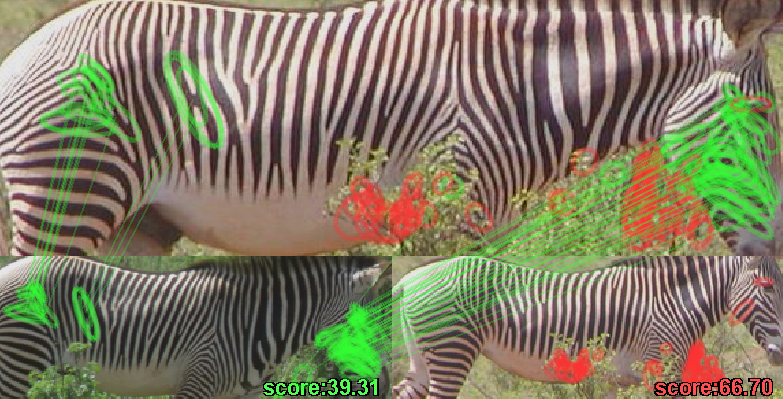
\includegraphics[width=.9\linewidth]{figures/FinalImages/cropped/GZ_incorrectRank4_443_cropped_fix}
\\
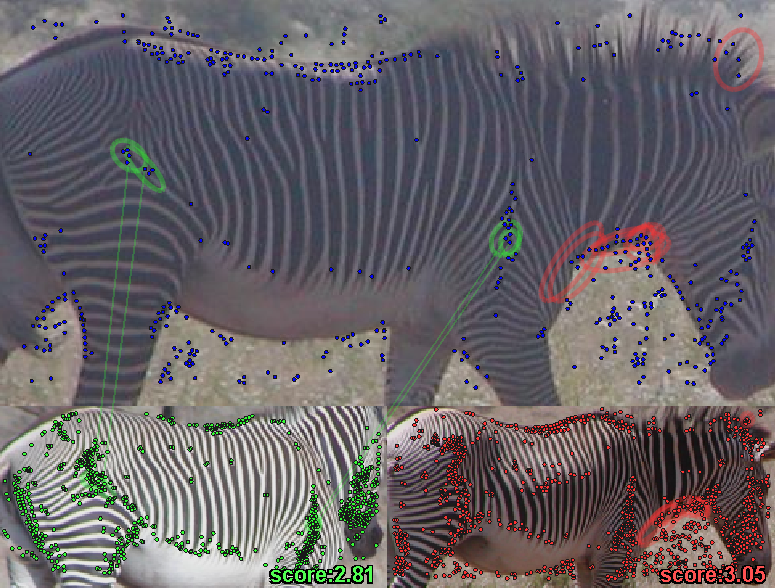
\includegraphics[width=.9\linewidth]{figures/FinalImages/cropped/GZ_incorrectRank2_501_cropped}
\\
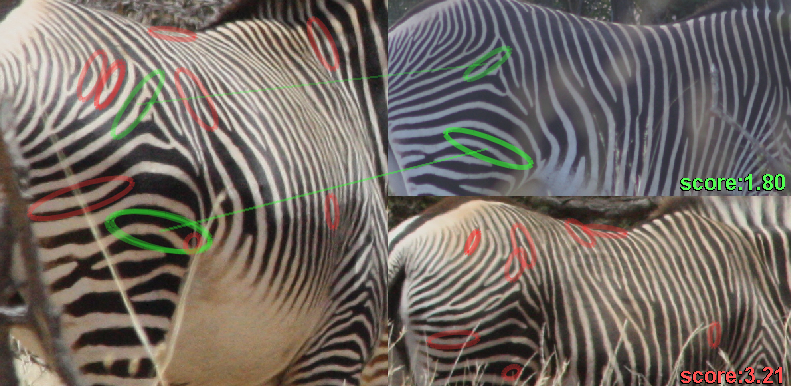
\includegraphics[width=.9\linewidth]{figures/FinalImages/cropped/GZ_incorrectRank6_1048_cropped_2}%Pose GZ
\end{tabular}
\caption{\footnotesize{Three example failures.  In the top example, the same
  background is seen (red matches) in two images showing different zebras.  In
  the middle, the viewpoints are too different between the query image
  and the correct database image (green matches), and a different
  image is the top match.  On the bottom, the poor illumination of
  the query image produces too few keypoints (small circles in the
  images) for correct matching.}}
\label{fig:problem}
\end{center}
\end{figure}

Further insight into HotSpotter can be gained through an analysis of
failures.  We closely analyzed the 34 Grevy's queries which produce a rank greater than
one for one-vs-many with $k=5$ and $\delta={\textrm{\tt lnrat}}$.
In 2 cases the database contained a mislabeling, and in 5 cases the
ROI covered two animals and matched the unlabeled animal. In 13 other cases,
the background scenery was matched instead of the
foreground zebra region.  A classifier that weights a descriptor
according to how likely it is to be a zebra should fix this problem.
Of the remaining 14 cases, 8 failed because of substantial pose variations between query
and database zebras, and the rest because of image quality, including focus,
resolution and contrast.  Examples are shown in Figure \ref{fig:problem}.
